\documentclass[a4paper]{article}

\usepackage[a4paper, margin=0.5in]{geometry}
\usepackage{graphicx}
\usepackage[linesnumbered,ruled,vlined]{algorithm2e}
\usepackage{color,soul}
\usepackage[utf8]{inputenc}
\usepackage[T1]{fontenc}
\usepackage{textcomp}
\usepackage{amsmath, amssymb}
\usepackage{caption}
\usepackage{listings}
\usepackage[italian]{babel}

% figure support
\usepackage{tikz}
\usetikzlibrary{calc}
\usepackage{import}
\usepackage{xifthen}
\pdfminorversion=7
\usepackage{pdfpages}
\usepackage{transparent}
\usepackage[hidelinks]{hyperref}
\usepackage{multirow}

% provides the H option
\usepackage{float}

\pdfsuppresswarningpagegroup=1

\begin{document}
	\title{Project log - Robotica}
	\author{Augello Andrea \and Castiglione Francesco Paolo \and La Martina Marco}
	\maketitle
	\tableofcontents

	\section{Setup}\label{sec:Setup}
	\begin{tabular}{|l|r|}
		\hline
		\multirow{2}{4em}{OS} & Ubuntu 18.04 \\
							  & Ubuntu 20.04 \\ \hline
		\multirow{2}{6em}{ROS version} & melodic \\
									   & noetic \\ \hline
		Webots & R2020b revision 1\\ \hline
		\multirow{2}{11em}{Target hardware} & Raspberry Pi 4B \\
											& Raspberry Pi 3B+ \\ \hline
	\end{tabular}

	\section{Nome}\label{sec:Name}
	Il team ha scelto il nome \textbf{Change} in onore di \textbf{Chang'e 4} \cite{change4}, la missione parte della seconda fase del programma cinese di esplorazione lunare, durante il quale è andato a buon fine il primo atterraggio morbido sulla faccia nascosta della luna. 

	\section{Ambiente}\label{sec:Libraries}
	Abbiamo considerato opportuno analizzare e studiare il package \textbf{webots\_ros} \cite{webotsRos} al fine di raggiungere una comprensione più profonda sulle metodologie per interfacciare i nodi ROS con il controller ROS standard per Webots. Inoltre è risultato necessario approfondire la documentazione ROS \cite{rosTutorial} al fine di installare e configurare l'ambiente ROS ed inoltre per capire i concetti fondamentali relativi ai nodi e topics. Infine abbiamo impostato l'interfaccia ROS su Webots seguendo la documentazione cyberbotics rilevante \cite{rosTutorial}.
	
	\section{Dipendenze}
	La seguente è una lista delle librerie utilizzate nel nostro progetto ed una breve spiegazione della loro funzione e rilevanza:
	
	\begin{itemize}
		\item opencv 4.x, una libreria per la computer vision, usata per operazioni di segmentazione \cite{opencv};
		\item imutils, che include funzioni per semplici operazioni di image processing quali traslazioni, rotazioni, ridimensionamento. Utilizzato inoltre per effettuare Non Maxima Suppression(NMS) \cite{imutils};
		\item sklearn, una libreria per il machine learning comprendente algoritmi di clustering quali DBSCAN \cite{scikit};
		\item numpy, una libreria che fornisce supporto per array multidimensionali, matrici ed operazioni matematiche per lavorare su detti array \cite{numpy};
		\item matplotlib, una libreria per creare visualizzazioni di dati (statiche, dinamiche, interattive) \cite{matplotlib};
		\item math, una libreria che fornisce funzioni matematiche definite dallo standard C \cite{math}.
	\end{itemize}

	\section{Obbiettivo}
	L'obbiettivo del robot è di \textbf{evitare assembramenti in ambienti indoor}. \newline
	Nella dimostrazione presentata il nostro robot rileva le persone nella stanza e individua i possibili assembramenti. In seguito alla fase di rilevazione si sposterà verso l'assembramento evitando gli ostacoli e, arrivato, esorterà le persone al rispetto del distanziamento sociale.
	
	\section{TIAGo Iron} 
	Il robot scelto per l'obbiettivo proposto è il \textbf{TIAGo Iron}. \newline Il \textbf{PAL Robotics TIAGo Iron} \cite{tiagoiron} è un robot umanoide a due ruote con torso e testa ma senza braccia articolate. Il modello è una piattaforma modulare mobile che permette l'interazione fra esseri umani e robot. \newline
	Abbiamo ritenuto necessario per il nostro scopo aggiungere uno \textbf{speaker} e un \textbf{display} con corrispondente solido di supporto al modello base del \textbf{TIAGo} disponibile in Webots.
	Inolte è stato necessario contattare gli sviluppatori di Webots per chiedere informazioni circa le dimensioni esatte delle \textbf{ruote} in quanto il modello Webots non corrisponde perfettamente alle specifiche indicate nel datasheet \cite{Tiago IRON datasheet}. Le ruote del modello hanno raggio di 200mm. 
	
    L'IMU utilizzata ha 6 gradi di libertà ed è composta delle seguenti componenti:
	\begin{enumerate}
		\item giroscopio;	
		\item accelerometro;
	\end{enumerate}
	Abbiamo ritenuto non necessario aggiungere il \textbf{magnetometro} in quanto in uno scenario reale sarebbe stato soggetto ad interferenze (significativamente più di un giroscopio), specialmente in un ambiente con molti oggetti metallici (quale potenzialmente lo scenario di utilizzo del nostro robot).

	\section{Modello del moto e posizionamento}
	Il modello del moto è caratterizzato da rotazioni e traslazioni. Per ottenere l'angolo di rotazione ci basiamo sui dati ottenuti dal giroscopio, il quale misura il moto rotazionale fornendo una velocità angolare. Per ottenere l'angolo di rotazione effettuiamo quindi un'integrazione discreta dei campioni con interpolazione lineare del primo ordine.
	Per effettuare lo spostamento lineare utilizziamo il controllore PID (Proporzionale-Integrale-Derivativo) delle ruote fornito da Webots, che richiede l'angolo di rotazione corrente, il diametro delle ruote e fornisce l'angolo di rotazione necessario al fine di ottenere lo spostamento desiderato.
	\begin{equation}\label{eq:odometry}
	targetAngle =
	currentAngle+2\pi\frac    {distance}
	{2\pi \cdot diameter}
	\end{equation}
	
	A causa di possibili imprecisioni calcoliamo la stima dello spostamento lineare utilizzando l'accelerometro. Al segnale dell'accelerometro viene applicato un integrale doppio per ottenere lo spostamento lineare.
	
	\section{Object recognition}
	Al fine di riconoscere le persone è stato necessario utilizzare sistemi di \textbf{object recognition}. A tal fine abbiamo valutato le performance di YOLOv3 (You only look once), YOLOv3-tiny, Hog (Histogram of gradients), Hog + SVG (Support Vector Machines) + NMS (Non Maxima suppression).
	In seguito a vari test su Hog abbiamo ritenuto essere problematica la larghezza delle bounding boxes fornite, in quanto, per motivazioni che verranno chiarite nel paragrafo successivo, vogliamo che queste ultime siano il più possibili vicile alla reale larghezza delle persone. YOLOv3, nonostante sia stato addestrato su foto di persone reali (e non modelli 3D) fornisce risultati soddisfacenti, in seguito al finetuning degli iperparaemtri parametri della rete. Tuttavia, considerando le caratterisiche hardware del robot mobile, abbiamo optato per l'uso di YOLOv3, il quale risulta essere significativamente più efficiente, sacrificando in termini di precisione ma comunque sufficientemente preciso per il nostro obbiettivo. Ecco un paragone fra YOLOv3 e YOLOv3-tiny in termini di mAP (mean average precision) e FLOPS (floating-point operations per second), come illustrato dalla tabella seguente, i cui dati provengono dal sito di YOLO \cite{yolo}:
	
	\begin{center}
		\begin{tabular}{ |c|c|c|c| } 
			\hline
			Model & mAP & FLOPS & FPS \\
			\hline
			\multirow{5}{4em} 							\\
			 YOLOv3-320    & 51.5  &  38.97  Bn  &  45  \\ 
			 YOLOv3-416    & 55.3  &  65.86  Bn  &  35  \\ 
			 YOLOv3-608    & 57.9  &  140.69 Bn  &  20  \\ 
			 YOLOv3-tiny   & 33.1  &  5.56   Bn  &  220 \\
			 YOLOv3-spp    & 60.6  &  141.45 Bn  &  20  \\
			\hline
		\end{tabular}
	\end{center}

	\section{Projection Matrix}
	\cite{OpenGL}
	
	\section{Clustering}
	We decided to lower the dimensionality of our data. We used cylindrical coordinates and the feature vector is 2 dimensional.
	We used the Density-Based Scan with a threshold. The entities not belonging to the cluster are discarded.
	
	\section{ROS}
	
	\section{Bugs found in the Webots ROS Controller}
	Logical values did not allow callbacks.
	

	\section{Distance calculation}\label{sec:Distance-calculation}
	The perceived object height is not a reliable indicator of its distance
	since part of the object may be occluded or not present in the frame.
	Moreover, some classifiers like the HoG based ones tend to produce ROIs
	significantly taller than the object.
	
	The torso width, on the other hand, is less susceptible to these issues,
	and does not depend on the pose (e.g. sitting vs standing). We however need
	to assume a cylindrical torso, introducing some error if the target is not
	facing the camera.

	The horizontal position of the object relative to the camera can influence
	its perceived width, shrinking it the further it is from the center of the
	image.  Assuming that a camera has a FOV of $2\alpha$ and has a distance
	$d$ from the object, the maximum horizontal distance a point in the image
	can have from the center of the image plane is $a = d \tan alpha$
	(Fig.~\ref{fig:error}).

	\begin{figure}[htpb]
		\centering
		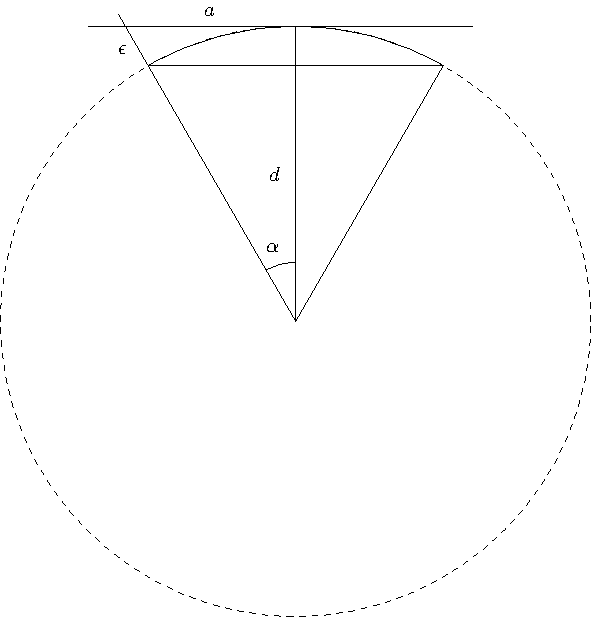
\includegraphics[width=0.8\textwidth]{./img/linearization_error.pdf}
		\caption{Error in distance estimate with piecewise circle linearization}
		\label{fig:error}
	\end{figure}

	Ignoring the perspective means performing a first order linear
	approximation and treating the point as if it lies in a circumference
	centered on the camera with $d$ as its radius. Hence, we consider the point
	being closer, committing the error shown in Eq.~\ref{eq:max_err}. With a
	camera FOV of 1 radiant as with the TIAGo this means that the maximum error
	due to the linearization amounts to a 13.9\% underestimate.

	\begin{equation}
		\epsilon = 
		\sqrt{a^2+d^2} - d =
		\sqrt{(d\tan \theta )^2+d^2}-d =
		d\left( \sqrt{\frac{1}{\cos ^2 \alpha}}-1 \right) =
		d \left( \sec \alpha -1 \right) 
		\label{eq:max_err}
	\end{equation}


	Under these assumptions we can compute the distance of an object as shown in
	Eq.~\ref{eq:obj_dist}

	\begin{equation}\label{eq:obj_dist}
		object~distance(m) = 
		\frac{f(m) \times real~width(m) \times image~width(pixels)}
			{object~width(pixels) \times sensor~width(m)}
	\end{equation}

	Since we are using a simulator, there is no camera sensor with a width to
	plug inside eq.~\ref{eq:obj_dist}. By placing both the robot and an object
	with known size in known positions and using this data together with pixel
	measurements in eq.~\ref{sensor_size}, we estimated the virtual sensor size
	to be used in all following computations.

	\begin{equation}\label{sensor_size}
		sensor~width(m) = 
		\frac{f(m) \times real~width(m) \times image~width(pixels)}
			{object~width(pixels) \times object~distance(m)}
	\end{equation}

	\newpage
	% Bibliography
	\bibliographystyle{unsrt}
	\begin{thebibliography}{19}
		\bibitem{tiagoiron} 
		\textit{https://cyberbotics.com/doc/guide/tiago-iron}. \newline
		Webots TIAGo Iron documentation.
		\bibitem{change4} 
		\textit{https://www.theguardian.com/science/2019/jan/03/china-probe-change-4-land-far-side-moon-basin-crater}. \newline
		The Guardian, 3 January 2019.
		\bibitem{webotsRos} 
		\textit{https://github.com/cyberbotics/webots\_ros}. \newline
		Github page for the \texttt{webots\_ros} package from \textit{cyberbotics}.
		\bibitem{rosTutorial} 
		\textit{https://wiki.ros.org/ROS/Tutorials}. \newline
		ROS documentation from ROS.org.
		\bibitem{webotsRosSetup} 
		\textit{https://www.cyberbotics.com/doc/guide/tutorial-8-using-ros}. \newline
		Cyberbotics documentation.
		\bibitem{Tiago IRON datasheet} 
		\textit{https://pal-robotics.com/wp-content/uploads/2019/07/Datasheet\_TIAGo\_Complete.pdf}. \newline
		Tiago IRON datasheet.
		\bibitem{OpenGL} 
		\textit{https://www.songho.ca/opengl/gl\_projectionmatrix.html}. \newline
		OpenGL Projection Matrix.
		\bibitem{positioning} 
		\textit{https://www.nxp.com/docs/en/application-note/AN3397.pdf}. \newline
		Implementing Positioning Algorithms Using Accelerometers.
		\bibitem{gmapping} 
		\textit{https://people.eecs.berkeley.edu/~pabbeel/cs287-fa11/slides/gmapping.pdf}. \newline
		Gmapping from UC Berkeley EECS, Pieter Abbeel.
		\bibitem{opencv} 
		\textit{https://opencv.org/}. \newline
		OpenCV Website.
		\bibitem{imutils} 
		\textit{https://github.com/jrosebr1/imutils}. \newline
		Imutils GitHub page.
		\bibitem{scikit} 
		\textit{https://scikit-learn.org/stable/}. \newline
		Scikit-learn website.
		\bibitem{numpy} 
		\textit{https://numpy.org/}. \newline
		Numpy website.
		\bibitem{matplotlib} 
		\textit{https://matplotlib.org/}. \newline
		Matplotlib website.
		\bibitem{math} 
		\textit{https://docs.python.org/3/library/math.html}. \newline
		Python documentation.
		\bibitem{yolo} 
		\textit{https://pjreddie.com/darknet/yolo/}. \newline
		Yolo website.
	\end{thebibliography}

\end{document}
